\chapter{Metodologia}
\label{cap-metodologia}
Este capítulo aborda sobre tudo que compõe a metodologia de pesquisa,
procedimentos e técnicas utilizados no trabalho, a fim de
explicar como o desenvolvimento do trabalho foi realizado para atingir os seus objetivos,
servindo como base para a sua reprodução em trabalhos futuros.

A pesquisa é fundamentada e metodologicamente construída objetivando a resolução
ou o esclarecimento de um problema. O problema é o ponto de partida da pesquisa.
Da sua formulação dependerá o desenvolvimento da sua pesquisa
\cite{moresi2003metodologia}, neste trabalho a questão problema a ser resolvida neste trabalho é:

\begin{center}
  \textit{
  Como implantar múltiplas aplicações a partir de um pacote único
  de forma centralizada e segura?
}
\end{center}

Para responder a questão problema deste trabalho se faz a necessidade de uma especificação
de uma metodologia de pesquisa que de acordo com \cite{marconi2002tecnicas} a
especificação da metodologia serve para abrangir itens que respondam as questões
Como? Com quê? Onde? De acordo com \cite{gerhardt2009metodos} existem diferentes tipos de pesquisa,
elas podem ser classificados quanto sua abordagem, sua natureza, seus objetivos e
seus procedimentos. Por isso é importante selecionar a modalidade de pesquisa
adequada ao objeto de pesquisa.

Assim este trabalho é classificado quanto à natureza como pesquisa aplicada
pois tem como objetivo gerar conhecimentos para aplicação prática, dirigidos à
solução de problemas específicos \cite{gerhardt2009metodos}. Quanto a abordagem,
a pesquisa é classificada como qualitativa, pois os pesquisadores que utilizam os
métodos qualitativos buscam explicar o porquê das coisas, exprimindo o que convém
a ser feito, mas não quantificam os valores nem nem se submetem a prova de fatos,
pois os dados analisados são não-métricos \cite{gerhardt2009metodos}.

Quanto aos objetivos, esta pesquisa é classificada como pesquisa descritiva, que
exige do investigador uma série de informações sobre o que deseja pesquisar.
Esse tipo de estudo pretende descrever os fatos e fenômenos de determinada realidade
\cite{trivinos1987introduccao}. Quanto aos procedimentos técnicos, serão utilizados
neste trabalho a pesquisa bibliográfica baseada no levantamento de referências
teóricas em livros e artigos científicos, permitindo conhecer o que já foi abordado
no assunto com trabalhos relacionados e conhecimentos prévios sobre a respeito da
possível solução à questão problema. Além disso também será usado a pesquisa
experimental que dado a proposta de solução da questão de pesquisa terá sua
validação baseada em exemplos de uso, cada um com o cenário de uso diferente para
testar a solução proposta.

Quanto às técnicas de coleta de dados, de acordo com \cite{gerhardt2009metodos}
a coleta de dados é a busca por informações para a elucidação do fenômeno ou
fato que o pesquisador quer desvendar, serão utilizados neste trabalho a pesquisa
bibliográfica e observação simples da execução da solução nos exemplos de uso.
A figura \ref{fig:metodologia1} apresenta de forma resumida a classficação da pesquisa

\begin{figure}[h]
  \centering
  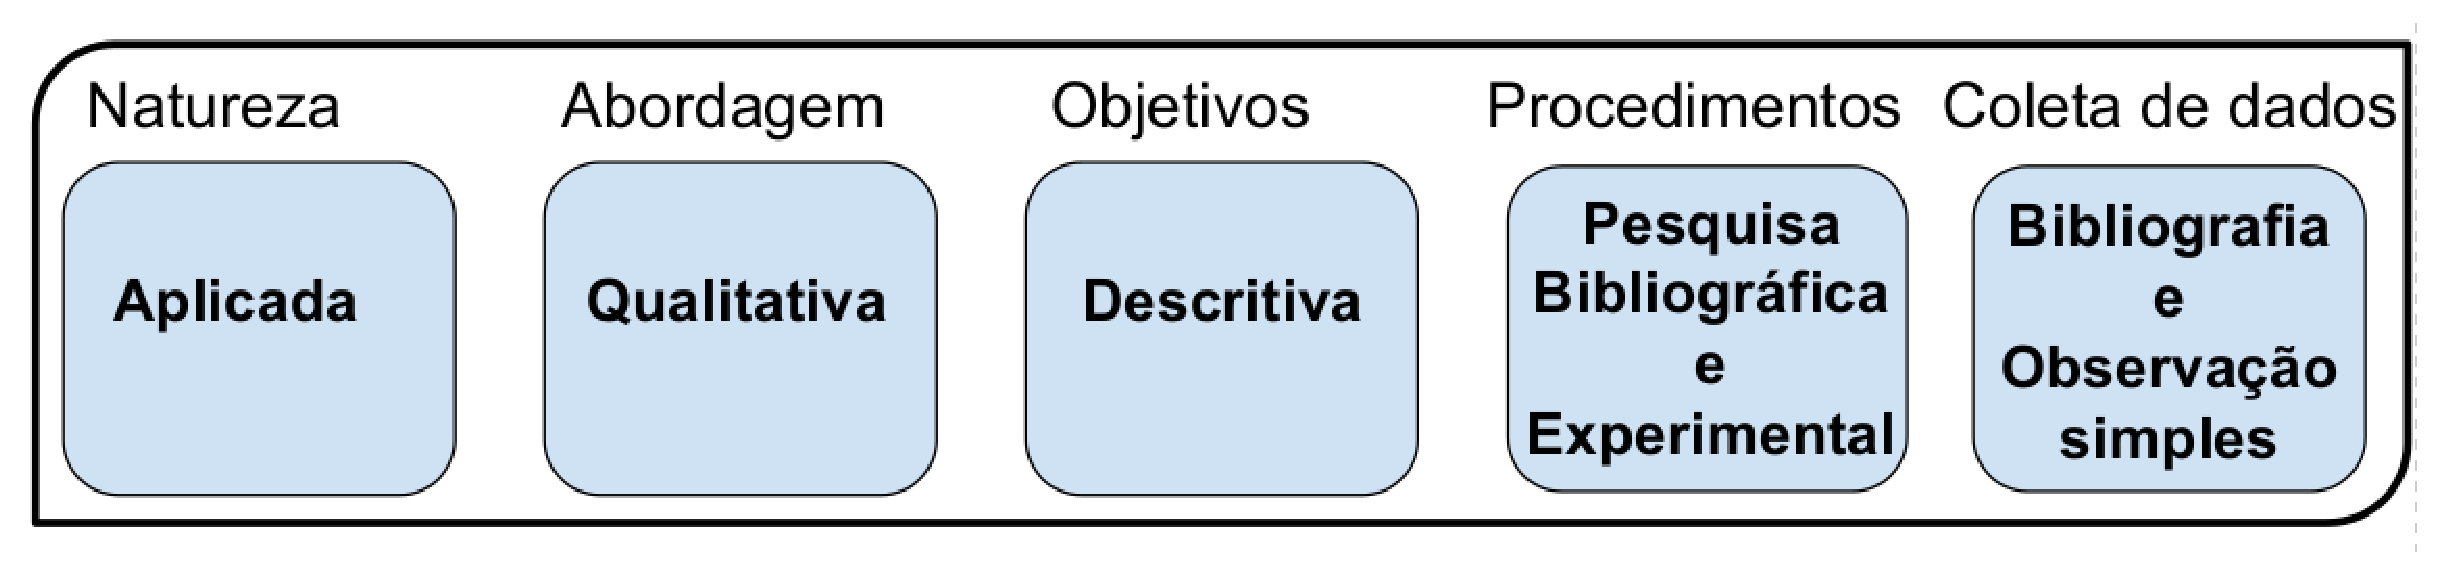
\includegraphics[width=1.0\textwidth]
      {figuras/metodologia1.eps}
  \caption{Resumo da classificação de pesquisa}
  \label{fig:metodologia1}
\end{figure}

Segundo \cite{andre2008estudo} uma pesquisa é executada de acordo com três fases:
Planejamento, Coleta de dados e Análise de dados. A fase de planejamento consiste
em definir o escopo do estudo junto com a questão de pesquisa, e a metodologia
de pesquisa com os seus procedimentos e exemplos de uso. Na fase de coleta de dados
se aplicam as técnics de coleta de dados definidas para que na última fase esses
dados sejam analisados e os resultados possam ser divulgados. Essas fases estão
resumidas na figura \ref{fig:metodologia2}.

\begin{figure}[H]
  \centering
  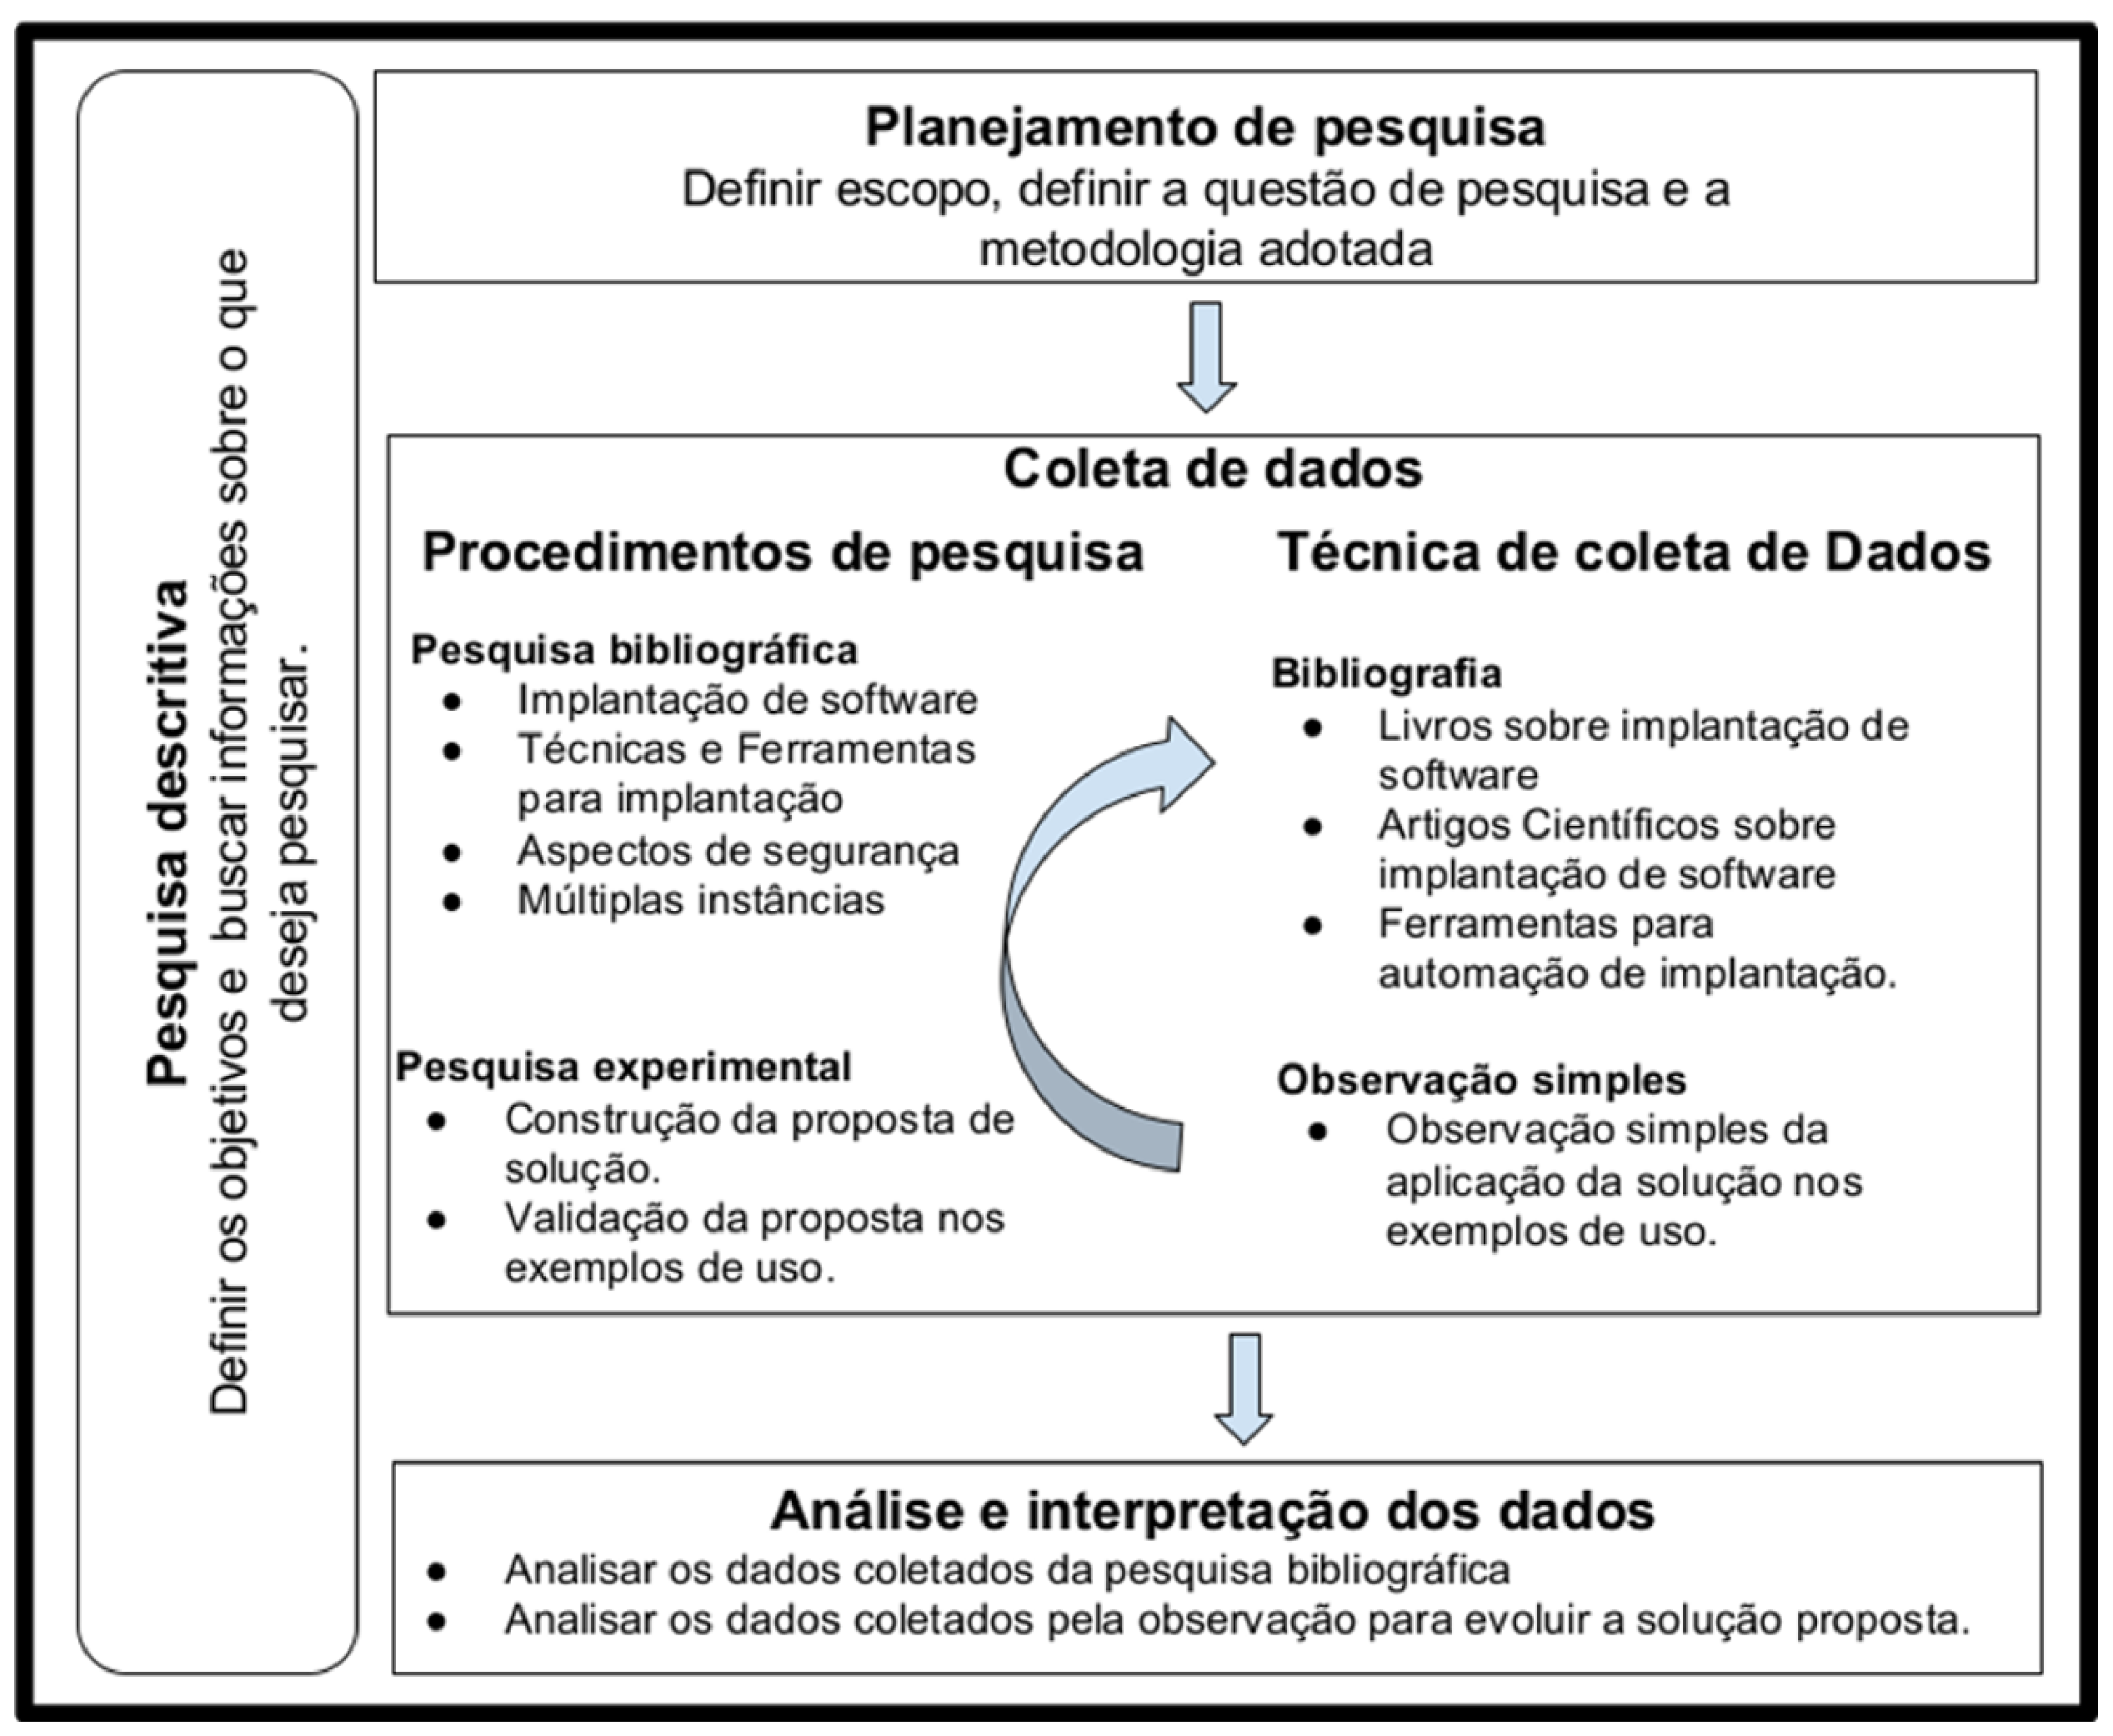
\includegraphics[width=1.0\textwidth]
      {figuras/metodologia2.eps}
  \caption{Fases da pesquisa}
  \label{fig:metodologia2}
\end{figure}

\section{Trabalhos Relacionados}

Para responder a questão problema primeiramente deve ser feito um levantamento
de trabalhos relacionados, para entender melhor como a automação da implantação
de software está sendo utilizada como solução na academia e nas empresas, e
quais são os procedimentos e técnicas utilizados, e se os aspectos de segurança
são levados em consideração.

Para entender o que acontece na comunidade da computação em relação a implantação
automatizada de aplicações, foi feito uma busca de alguns trabalhos relacionados, o primeiro
trabalho relacionado é um trabalho acadêmico feito por \cite{leo2014} no qual foi
desenvolvido um sistema de middleware chamado CHOReOS Enactment Engine que é um
sistema que possibilita a implantação distribuída e automatizada de composições
de serviços web em uma estrutura virtualizada, no qual opera no modelo
computacional conhecido como plataforma como serviço, comparando esse sistema
com abordagens ad-hoc de implantação levando em consideração a escalabilidade
em relação ao tempo de implantação das composições dos serviços.

Existem também ferramentas disponíveis no mercado que também trazem a proposta
de automação de instalação de aplicações alguns exemplos são: \cite{bitnami}
BitNami que é uma biblioteca de aplicativos de servidor populares e ambientes de
desenvolvimento que pode ser instalado com um clique. Ele automatiza todo o
processo de compilar e configurar os aplicativos e todas as suas dependências
(bibliotecas de terceiros, linguagem de programação, bases de dados) para que o
usuário comum não se preocupe com questões mais técnicas. Também temos o
\cite{sandstormio} Sandstorm é uma plataforma de código aberto para servidores
pessoais. Sandstorm permite que você execute o seu próprio servidor e instalar
facilmente as aplicações em que dão suporte, e por fim a ferramenta \cite{juju}
Juju que lhe permite implementar,configurar, gerenciar, manter e serviços de forma
rápida e eficiente automatizando a instalação e configuração de aplicações na nuvem.

O estudo dessas aplicações serve como base para entender como são feitas as
arquiteturas que são utilizadas pela comunidade da computação, por exemplo o JuJu
utiliza uma abstração conhecida como charm, que são o códigos que define um serviço,
um charm contém toda a lógica de que você precisa para implementar e integrar uma
aplicação, contendo todo o processo de download de ferramentas, instalação e configuração
de aplicações, podendo ser escrito
em várias linguagens ou até provisionadores como chef, puppet ou docker \cite{juju}, é
possível reaproveitar os charms feitos pela comunidade do JuJu assim reaproveitando
os charms prontos ou não precisando escrever um charm do zero.

Já bitnami ja tráz as aplicações
prontas pra uso, assim o usuário interage no formato clique para instalar, porém o usuário
só tem a disposição as aplicações disponibilizadas pelo bitnami, isso também é
a forma em que o sandstorm.io trabalha, com a diferença de que o standstorm é
software livre. Já o trabalho feito por \cite{leo2014} é voltado para serviços web
de grande escala, com foco em implantação de aplicações na nuvem e escalar infraestrutura, utilizando o middleware
construido em seu trabalho, assim podendo gerenciar ambientes de computação em nuvem
como Amazon EC2 e Openstack, sua engine utiliza o chef solo como seu agente de configuração.

Com esse levantamento vemos que existem soluções bem próximas do que este trabalho
pretende atingir como objetivo, assim temos como hipótese que é possível construir
uma arquitetura que atinja o objetivo deste trabalho que é automatizar instalação e configuração de
múltiplas instâncias de uma aplicação web utilizando pacotes debian.

Visto que a utilização do empacotamento traz inúmeras vantagens no processo de implantação
de aplicações como citado no capítulo \ref{cap-introducao}, tendo o levantamento dos trabalhos relacionados
e a questão de pesquisa como insumo, e a hipótese levantada, justifica-se a
definição de uma proposta de arquitetura e procedimentos para implantação automatizada
de aplicações web que utilizam pacotes debian.

\section{Procedimentos para proposta de arquitetura}

A partir do referencial teórico é possível definir uma proposta de
arquitetura básica para implantação automatizada de aplicações definindo as
tecnologias utilizadas, ferramentas escolhidas para compor a arquitetura e procedimentos
a serem seguidos que levam em consideração as boas práticas de implantação e os
aspectos de segurança na implantação de software. Na definição da arquitetura inicial
é importante levar em consideração os seguintes aspectos:

\begin{itemize}
  \item  \textbf{A1 :} Aspectos de segurança na implantação de aplicações web.
  \item  \textbf{A2 :} Aspectos para implantação automatizada de múltiplas instâncias de
   aplicações no mesmo servidor.
  \item  \textbf{A3 :} Possibilidade de lidar com aplicações desenvolvidas em
  diferentes linguagens.
  \item  \textbf{A4 :} Aplicações que são empacotadas no debian.
  \item  \textbf{A5 :} Boas práticas de implantação de software.
\end{itemize}

Esses aspectos são importantes para definir o que vai compor a arquitetura inicial,
para que se possa validar a proposta com os exemplos de uso,
podendo assim evoluir a arquitetura proposta. Além disso também é preciso definir
alguns procedimentos importantes para a construção da arquitetura inicial
considerando o processo de implantação de software visto no
capítulo \ref{cap-introducao} e a referência dos trabalhos relacionados, os procedimentos
são os seguintes:

\begin{itemize}
  \item  \textbf{Definir tecnologia para automatizar implantação :}  Definir qual será a
  tecnologia escolhida dentre as citadas no referencial teórico para dar suporte
  a implantação.
  \item  \textbf{Definir conjunto mínimo de dependências:} Definir quais são as dependências
  mínimas para o funcionamento de uma aplicação independente das aplicações escolhidas para
  servir de exemplos de uso, tais como: sistema operacional, pacotes pré-instalados
  e aplicações pré-configuradas, como por exemplo: servidor web e banco de dados.
  \item  \textbf{Definir as fases e os procedimentos para implantação automatizada:}
   Definir quais são etapas da implantação, definir a ordem necessária para a execução de
  cada fase da implantação, dado a importância de definir as fases que compõem o processo de
  implantação e de acordo com \cite{omg2006}.
  \item  \textbf{Definir os aspectos de segurança} Definir quais são os aspectos de segurança
  e automatizar os que forem possíveis de serem aplicados dentro do contexto da arquitetura
  proposta.
\end{itemize}

Com a arquitetura definida o próximo passo é definir um ambiente de desenvolvimento e de
testes, dado o contexto de implantação de software é importante possuir um ambiente flexível para
testar facilmente a instalação e configuração das aplicações e podendo facilmente
reinicializar esse ambiente de forma que ele fique limpo sem resquícios da instalação
anterior. Com a arquitetura definida e com um ambiente de desenvolvimento e de testes configurados, é
necessário definir quais são as aplicações que servirão como caso de testes
para a implementação da solução. Elas serão importantes pois a partir delas
e de suas necessidades que será feito a validação da proposta e seus refinamentos.

\section{Validação da proposta}

Para validar a arquitetura proposta no trabalho serão feitos exemplos de uso com aplicações
que possam servir como base para validação da proposta de arquitetura, a fim de
refinar e evoluir a solução, baseada em exemplos de uso com aplicações reais e conhecidas
na comunidade de software livre, devem ser levados as seguintes características para a
escolha das aplicações:

\begin{itemize}
  \item  \textbf{Aplicações empacotadas no debian :}  Como o intuito do trabalho
  é realizar implantações múltiplas a partir de um pacote único, tais aplicações
  devem estar empacotadas e disponíveis para instalação nos servidores do debian.
  Isso impacta na escolha da ferramenta, visto que não será necessário ter o trabalho
  de empacotar aplicações que ainda não estão empacotadas no debian.
  \item  \textbf{Servidor web compatível:} As ferramentas escolhidas devem no
  mínimo possuir o servidor web compatível, por exemplo: as aplicações juntas
  devem possuir suporte para nginx ou apache ou similares.
  \item  \textbf{Aplicações com comunidades ativas:} Como estamos trabalhando
  com software livre, é importante que os softwares escolhidos possuem comunidades
  ativas, isso pode ajudar na resolução de  possíveis problemas, logo aplicações
  em que sejam difíceis de comunicar com sua comunidade devem ser evitadas, e
  aplicações com a comunidade de desenvolvedores e usuários ativa devem ser priorizadas.
  E isso também pode ser um fator importante caso durante os testes sejam descobertos
  bugs ou melhorias dentro dessas ferramentas e tais bugs e melhorias possam ser
  reportados para a comunidade, ou até mesmo solucionados e devolvidos aos mantenedores
  das ferramentas.
  \item  \textbf{Documentação do software:} A documentação do software também deve
  ser levado em consideração, principalmente a documentação da instalação e configuração
  dentro da ferramenta, ferramentas que não possuem documentação de instalação e
  configuração devem ser evitadas.
\end{itemize}

\subsection{Exemplos de uso}

Para validar a arquitetura, serão escolhidos alguns exemplos de uso, com a
finalidade de verificar se com tais métodos e procedimentos atingirá o objetivo
estabelecido. Para a escolha das aplicações que serão utilizadas como exemplos
de uso é necessário fazer uma busca nas aplicações web que são empacotadas no
debian e que possuem suporte a configuração de múltiplas instâncias, essa busca
deve levar em consideração também a documentação para realizar tal configuração.
Foram levantados algumas aplicações web empacotadas no debian da seguinte forma:

\begin{center}
apt-cache search web | wc -l
\end{center}

O resultado obtido com pacotes que contenham a palavra web recebe o resultado de 3470
pacotes de diversas aplicações ou módulos de aplicações, como:
wordpress, owncloud, drupal, mailman, chromium, etc. Logo dentro dessa rápida busca
encontramos alguns pacotes de aplicações conhecidas, para facilitar a busca basta
aplicar para alguns nomes de aplicações conhecidos como:

\begin{center}
apt-cache search web | grep wordpress
\end{center}

Para avaliar se as aplicações possuem suporte a múltiplas instâncias é necessário
analisar a documentação das aplicações, as aplicações costumam disponibilizar a sua
documentação na sua página ou em uma wiki, também é possível checar a documentação
quando se instala uma aplicação nos arquivos de documentação da aplicação em
/usr/share/doc/ ou também pode-se utilizar os comandos:

\begin{center}
man nomeaplicação

info nomeaplicação
\end{center}

Com as aplicações que serão exemplos de uso escolhidas a proposta de arquitetura
pode ser testada e validada, com o objetivo de criar múltiplas instâncias
no mesmo servidor de forma automatizada a partir de um pacote único, logo os
exemplos de uso também servirão para refinar e evoluir a arquitetura proposta.
Para realizar tais validações é importante que as instalações e configurações
sejam em um ambiente limpo, ou seja, os testes devem ser criados de preferência
em máquinas virtuais com a configuração conhecida como "minimal", que contém
instalado apenas as aplicações necessárias para o funcionamento do sistema operacional.

A partir da execução dos exemplos de uso será possível a coleta de informações
necessárias para a validação da solução proposta, essa validação a princípio
será feita a partir da execução da implantação e verificação das funcionalidades
da aplicação implantada, ou seja, após a execução da implantação o testador deverá
verificar o perfeito funcionamento de algumas funcionalidades básicas da aplicação
escolhida, e principalmente verificar a implantação de várias instâncias da mesma
aplicação no mesmo servidor destino, observando o perfeito funcionamento de todas as
instâncias implantadas assim validando a implantação de múltiplas instâncias.
